\subsection{Langkah Praktikum: BFS dan DFS pada Graf 6.1}

\begin{figure}[H]
    \centering
    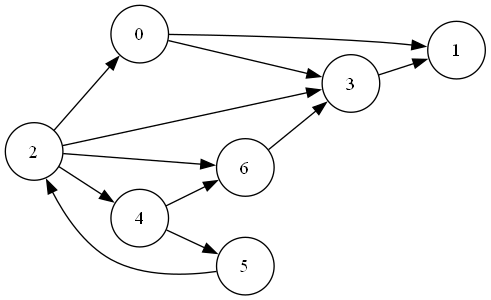
\includegraphics[width=0.65\textwidth]{figures/praktikum6/graf_praktikum.png}
    \caption{Visualisasi Graf Berarah Gambar 6.1 (Langkah Praktikum)}
\end{figure}

\subsubsection*{Flowchart BFS}
\begin{figure}[H]
    \centering
    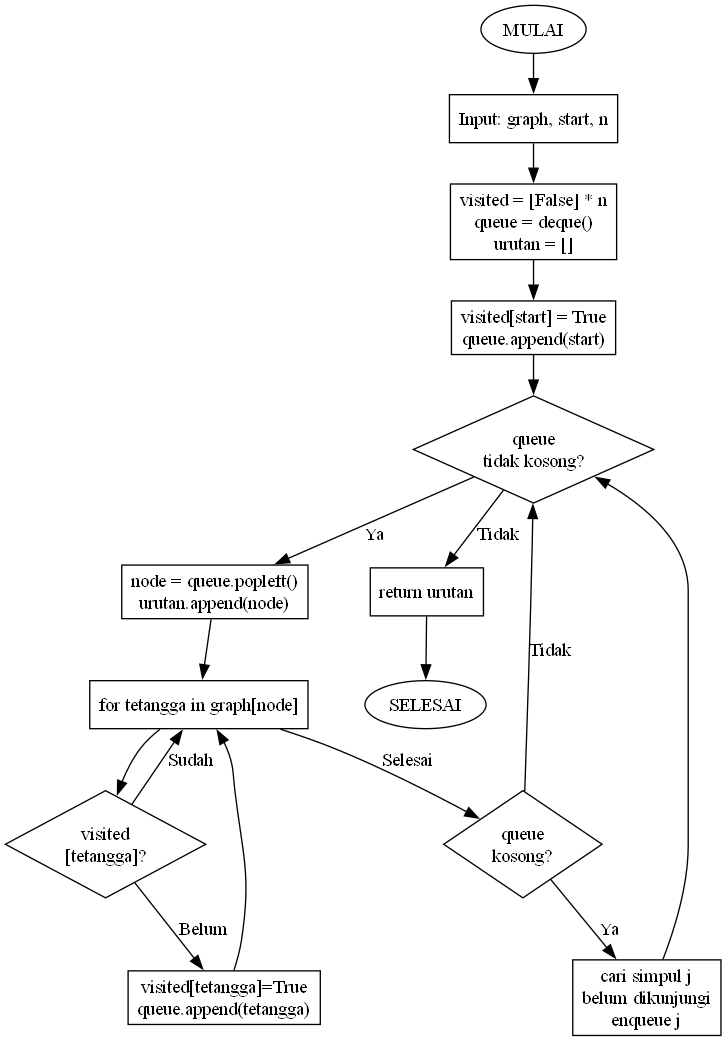
\includegraphics[width=0.45\textwidth]{figures/praktikum6/flowchart_bfs.png}
    \caption{Flowchart Algoritma BFS}
\end{figure}

\subsubsection*{Flowchart DFS}
\begin{figure}[H]
    \centering
    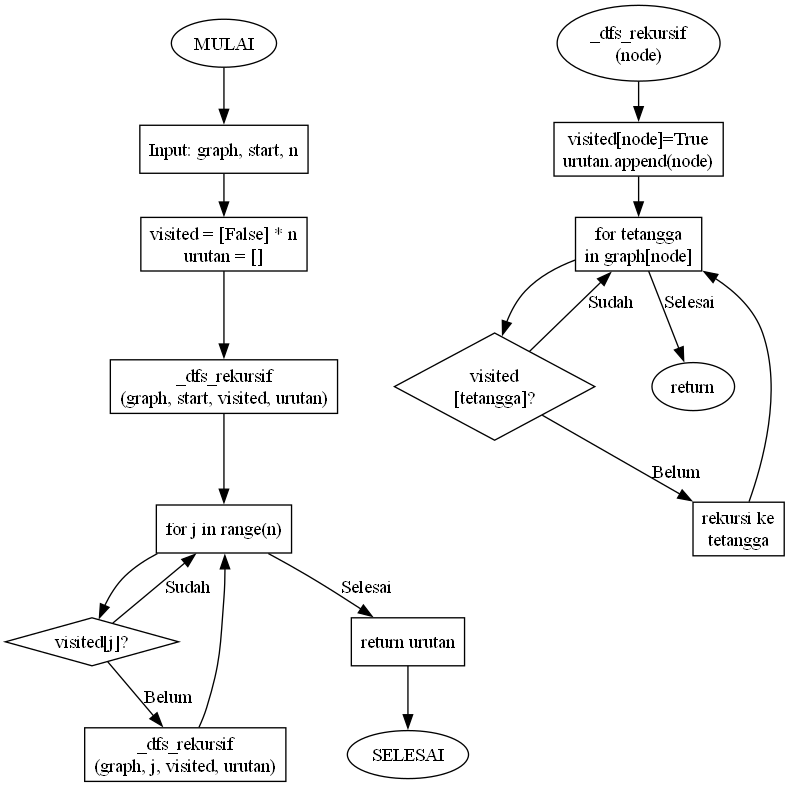
\includegraphics[width=0.45\textwidth]{figures/praktikum6/flowchart_dfs.png}
    \caption{Flowchart Algoritma DFS}
\end{figure}

\subsubsection*{Source Code Python: BFS}
\begin{lstlisting}[basicstyle=\ttfamily\scriptsize, frame=single, backgroundcolor=\color{white}, numbers=none, keywordstyle=\color{black}, commentstyle=\color{black}, stringstyle=\color{black}, breaklines=true]
def bfs(graph, start, n):
    visited = [False] * n
    urutan = []
    queue = deque()
    
    # tandai simpul awal sebagai dikunjungi dan masukkan ke antrian
    visited[start] = True
    queue.append(start)
    
    while queue:
        # ambil simpul paling depan antrian
        node = queue.popleft()
        urutan.append(node)
        
        # kunjungi semua tetangga yang belum dikunjungi
        for tetangga in graph[node]:
            if not visited[tetangga]:
                visited[tetangga] = True
                queue.append(tetangga)
                
        # jika antrian kosong tapi masih ada simpul yang belum dikunjungi
        if not queue:
            for j in range(n):
                if not visited[j]:
                    visited[j] = True
                    queue.append(j)
                    break
                    
    return urutan

if __name__ == "__main__":
    # graf berarah Gambar 6.1 sesuai kode tester modul
    n = 7
    graph = {
        0: [1, 3],
        1: [],
        2: [0, 3, 4, 6],
        3: [1],
        4: [5, 6],
        5: [2],
        6: [3],
    }
    hasil = bfs(graph, 0, n)
    print("BFS mulai dari node 0:", hasil)
\end{lstlisting}

\subsubsection*{Source Code Python: DFS}
\begin{lstlisting}[basicstyle=\ttfamily\scriptsize, frame=single, backgroundcolor=\color{white}, numbers=none, keywordstyle=\color{black}, commentstyle=\color{black}, stringstyle=\color{black}, breaklines=true]
def _dfs_rekursif(graph, node, visited, urutan):
    # tandai simpul saat ini sebagai dikunjungi
    visited[node] = True
    urutan.append(node)
    
    # kunjungi semua tetangga yang belum dikunjungi secara rekursif
    for tetangga in graph[node]:
        if not visited[tetangga]:
            _dfs_rekursif(graph, tetangga, visited, urutan)

def dfs(graph, start, n):
    visited = [False] * n
    urutan = []
    
    # mulai DFS dari simpul awal
    _dfs_rekursif(graph, start, visited, urutan)
    
    # tangani simpul yang belum terjangkau
    for j in range(n):
        if not visited[j]:
            _dfs_rekursif(graph, j, visited, urutan)
            
    return urutan

if __name__ == "__main__":
    # graf berarah Gambar 6.1 sesuai kode tester modul
    n = 7
    graph = {
        0: [1, 3],
        1: [],
        2: [0, 3, 4, 6],
        3: [1],
        4: [5, 6],
        5: [2],
        6: [3],
    }
    hasil = dfs(graph, 0, n)
    print("DFS mulai dari node 0:", hasil)
\end{lstlisting}

\subsubsection*{Analisis Output dan Perbedaan Kedua Algoritma}
Program dijalankan pada graf berarah Gambar 6.1 (7 simpul) dimulai dari node 0. Graf memiliki edge: 0$\rightarrow$1, 0$\rightarrow$3, 2$\rightarrow$0, 2$\rightarrow$3, 2$\rightarrow$4, 2$\rightarrow$6, 3$\rightarrow$1, 4$\rightarrow$5, 4$\rightarrow$6, 5$\rightarrow$2, 6$\rightarrow$3.

\begin{table}[H]
    \centering
    \caption{Perbandingan Urutan Traversal BFS dan DFS}
    \begin{tabular}{llp{3cm}p{3cm}}
    \toprule
    \textbf{Algoritma} & \textbf{Urutan Traversal} & \textbf{Simpul ke-5 dikunjungi ke-} & \textbf{Simpul ke-6 dikunjungi ke-} \\ \midrule
    BFS & [0, 1, 3, 2, 4, 6, 5] & ke-7 (terakhir) & ke-6 \\
    DFS & [0, 1, 3, 2, 4, 5, 6] & ke-6 & ke-7 (terakhir) \\ \bottomrule
    \end{tabular}
\end{table}

Perbedaan terlihat pada urutan kunjungan simpul 5 dan 6. BFS mengunjungi simpul 6 sebelum 5 karena 6 masuk antrian lebih dulu (saat memproses simpul 4, edge 4$\rightarrow$6 diperiksa sebelum 4$\rightarrow$5 jika indeks lebih kecil diutamakan). DFS sebaliknya, masuk ke simpul 5 terlebih dahulu mengikuti cabang 4$\rightarrow$5 sebelum backtrack ke 4$\rightarrow$6.

\subsubsection*{Visualisasi Urutan Traversal}

\begin{figure}[H]
    \centering
    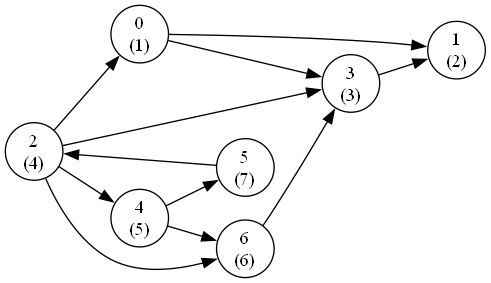
\includegraphics[width=0.65\textwidth]{figures/praktikum6/graf_bfs.png}
    \caption{Urutan BFS dari Node 0 (angka dalam kurung = urutan kunjungan)}
\end{figure}

\begin{figure}[H]
    \centering
    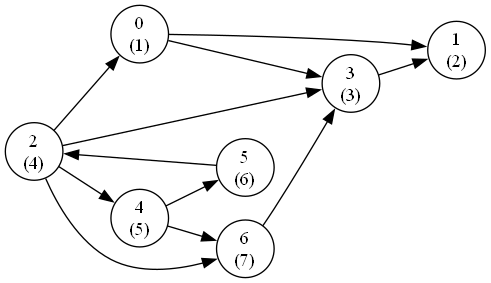
\includegraphics[width=0.65\textwidth]{figures/praktikum6/graf_dfs.png}
    \caption{Urutan DFS dari Node 0 (angka dalam kurung = urutan kunjungan)}
\end{figure}

\subsection{Post Test: BFS dan DFS pada Graf Pre Test (Gambar 6.4)}

\subsubsection*{Source Code Python}
\begin{lstlisting}[basicstyle=\ttfamily\scriptsize, frame=single, backgroundcolor=\color{white}, numbers=none, keywordstyle=\color{black}, commentstyle=\color{black}, stringstyle=\color{black}, breaklines=true]
from collections import deque

def bfs(graph, start, n):
    visited = [False] * n
    urutan = []
    queue = deque()
    
    # tandai simpul awal dan masukkan ke antrian
    visited[start] = True
    queue.append(start)
    
    while queue:
        node = queue.popleft()
        urutan.append(node)
        
        # kunjungi tetangga yang belum dikunjungi
        for tetangga in graph[node]:
            if not visited[tetangga]:
                visited[tetangga] = True
                queue.append(tetangga)
                
        # tangani simpul tidak terjangkau
        if not queue:
            for j in range(n):
                if not visited[j]:
                    visited[j] = True
                    queue.append(j)
                    break
                    
    return urutan

def _dfs_rekursif(graph, node, visited, urutan):
    # tandai dan catat simpul yang dikunjungi
    visited[node] = True
    urutan.append(node)
    
    # rekursif ke tetangga yang belum dikunjungi
    for tetangga in graph[node]:
        if not visited[tetangga]:
            _dfs_rekursif(graph, tetangga, visited, urutan)

def dfs(graph, start, n):
    visited = [False] * n
    urutan = []
    
    _dfs_rekursif(graph, start, visited, urutan)
    
    # tangani simpul yang belum terjangkau
    for j in range(n):
        if not visited[j]:
            _dfs_rekursif(graph, j, visited, urutan)
            
    return urutan
\end{lstlisting}

\textbf{Jawaban 1: Penerapan BFS dan DFS pada graf Gambar 6.4}\\
Program dijalankan pada graf pre test (Gambar 6.4) dengan 7 simpul mulai dari node 0:

\begin{table}[H]
    \centering
    \caption{Validasi Hasil Program vs Manual pada Graf Pre Test}
    \begin{tabular}{lllp{1.5cm}}
    \toprule
    \textbf{Algoritma} & \textbf{Hasil Program} & \textbf{Jawaban Manual Pre Test} & \textbf{Sama?} \\ \midrule
    BFS & [0, 1, 2, 3, 4, 5, 6] & [0, 1, 2, 3, 4, 5, 6] & Ya \\
    DFS & [0, 1, 3, 5, 2, 4, 6] & [0, 1, 3, 5, 2, 4, 6] & Ya \\ \bottomrule
    \end{tabular}
\end{table}

\textbf{Jawaban 2: Analisis kesesuaian hasil program dengan jawaban pre test}\\
Hasil program sepenuhnya sesuai dengan jawaban manual pre test untuk kedua algoritma. Ini memvalidasi bahwa:
\begin{enumerate}
    \item Implementasi Python BFS menggunakan \texttt{deque} sudah benar dalam mengeksplorasi graf secara berlapis, menghasilkan urutan yang identik dengan penelusuran manual menggunakan antrian.
    \item Implementasi Python DFS rekursif sudah benar dalam mengeksplorasi graf secara mendalam, menghasilkan urutan yang identik dengan penelusuran manual menggunakan prinsip backtracking.
    \item Penanganan simpul tidak terjangkau (isolated nodes) sudah ditangani dengan benar di kedua implementasi sehingga seluruh 7 simpul berhasil dikunjungi.
\end{enumerate}